% !TeX spellcheck = id_ID
\documentclass[a4paper,12pt]{article}
\usepackage[bahasa]{babel}
\usepackage{graphicx}
\usepackage{multirow}
\usepackage{enumitem}
\usepackage[T1]{fontenc}
\usepackage{inconsolata}
\usepackage{lipsum}
\usepackage{xcolor}

\graphicspath{ {./img/} }
\begin{document}
\title{ {\Large Laporan Praktikum}\\ Jaringan Komputer \\{\Large Pertemuan 10}}

\author{Aldzikri Dwijayanto Prathama 
	\\195410189
	\\Teknik Informatika}
\makeatletter
\begin{titlepage}
	\begin{center}
		{\huge \bfseries \@title }\\[14ex]
		
\includegraphics[scale=.8]{logo}\\[4ex]
		{\large \@author}\\[19ex]
		{\large \bfseries {SEKOLAH TINGGI MANAJEMEN INFORMATIKA DAN KOMPUTER
				AKAKOM YOGYAKARTA}}
	\end{center}


{\large \@date} 
\end{titlepage}
\makeatother
\newpage
\tableofcontents
\newpage

\section{Tujuan}
Mahasiswa mampu melakukan konfigurasi NAT untuk mengakses Internet

\section{Dasar Teori}
Penafsiran alamat jaringan (Network Address Translation atau NAT) adalah suatu
metode untuk menghubungkan lebih dari satu komputer ke jaringan Internet dengan
menggunakan satu alamat IP. Banyaknya penggunaan metode ini disebabkan karena
ketersediaan alamat IP yang terbatas, kebutuhhan akan keamanan (security), dan
kemudahan serta fleksibilitas dalam administrasi jaringan.

\begin{center}
	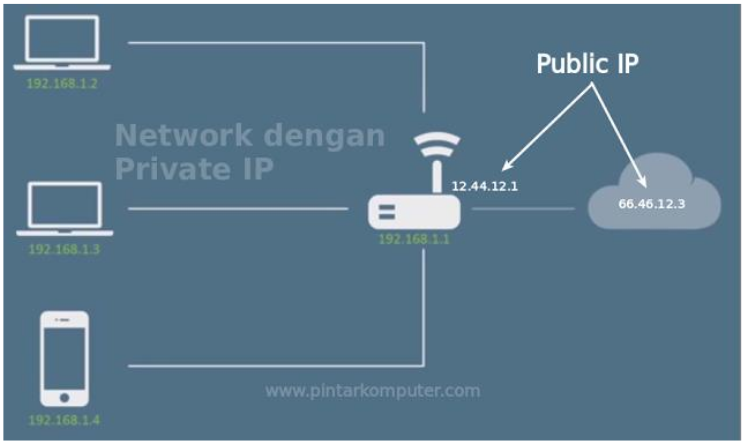
\includegraphics[scale=.3]{dasar}
\end{center}

\paragraph{Alamat IP yang terbatas\\}
Saat ini, IPv4 masih banyak digunakan. Oleh karena IPv4 menggunakan 32 bit,
maka secara teoritis hanya terdapat 2 32 alamat = 4.294.967.296 alamat IP saja. Karena
keterbatasan inilah sebagian besari ISP (Internet Service Provider) hanya akan
mengalokasikan satu alamat untuk satu pengguna dan alamat ini bersifat dinamik, artinya
alamat IP yang diberikan akan berbeda setiap kali user melakukan koneksi ke Internet,
akan tetapi juga hanya tersedia satu IP untuk satu komputer saja yang dapat terkoneksi
ke Internet. Hal ini dapat diatasi dengan menggunakan NAT. Dengan NAT gateway yang
dijalankan pada salah satu komputer, satu alamat tersebut dapat dibagi ke komputer lain
sehingga semuanya dapat terkoneksi ke Internet secara bersamaan.

\paragraph{Keamanan\\}
Ketika sebuah komputer terkoneksi ke Internet, komputer tersebut tidak hanya
terkoneksi ke salah satu server suatu situs tertentu, namun sangat mungkin juga diakses
oleh komputer lain yang juga terkoneksi ke Internet. Jika disalahgunakan, tentunya sangat
berbahaya. Data-data penting dapat dilihat dan dicuri oleh pihak lain. NAT secara otomatis
memberikan proteksi seperti halnya firewall dengan hanya mengijinkan koneksi yang
berada di dalam jaringan LAN.

\paragraph{Administrasi Jaringan\\}
Dengan NAT, suatu jaringan yang besar dapat dipecah-pecah menjadi jaringan-
jaringan yang lebih kecil. Bagian-bagian kecil tersebut memiliki satu alamat IP, sehingga
dapat menambahkan atau mengurangi jumlah komputer tanpa mempengaruhi jaringan
secara keseluruhan. Selain itu, pada gateway NAT modern terdapat server DHCP yangdapat mengkonfigurasi komputer client secara otomatis. Selain itu, gateway NAT dapat
membatasi akses ke Internet, juga mampu mencatat semua lalu lintas data, dari dan ke
Internet. Secara keseluruhan, dengan segala kelebihan gateway NAT tersebut, admin
jaringan akan sangat terbantu dalam melakukan tugas-tugasnya.

\section{Praktik}
\begin{enumerate}
	\item \textbf{Instalasi Jaringan}\\
	Langkah pertama adalah menyambungkan router dengan jaringan, port ether1 yang berperan sebagai dhcp client disambungkan ke jaringan internet akakom, lalu ether2 disambungkan ke pc1, sedangkan ether3 yang akan memiliki dhcp server disambungkan ke pc2. 
	
	\item \textbf{Menghapus konfigurasi Mikrotik}\\
	\begin{center}
		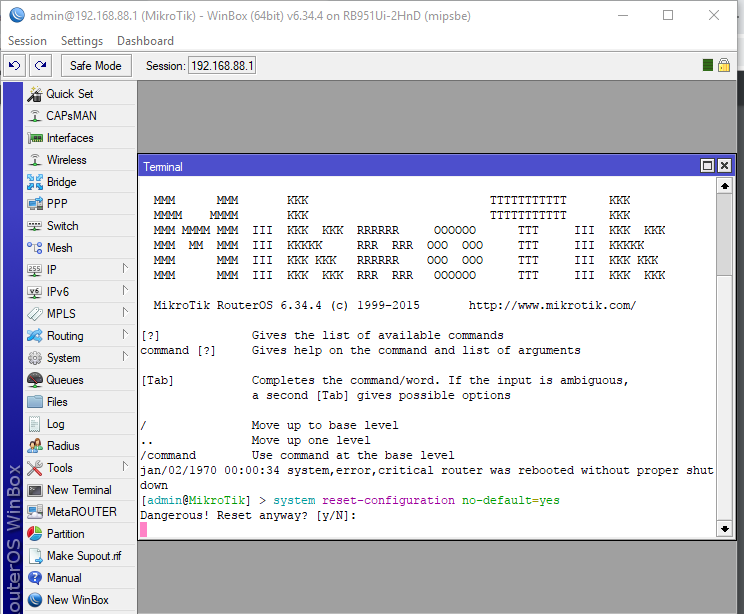
\includegraphics[scale=.4]{Capture1}
	\end{center}
	Untuk me-reset konfigurasi pada mikrotik, pertama login terlebih dahulu dengan winbox, lalu kilk new terminal dan tuliskan \texttt{system reset-configuration no-default=yes}, perintah tersebut akan mereset router tanpa konfigurasi default. Lalu tekan y untuk konfirmasi.Maka Mikrotik akan booting dan konfigurasinya telah dihapus semua. Lalu login kembali dengan mac address.
	
	\item \textbf{Cek IP Address pada Interface.\\}
	Klik menu IP → Addresses, maka akan muncul kotak windows Address List dan
	pastikan pada kotak tersebut masih kosong.
	\begin{center}
		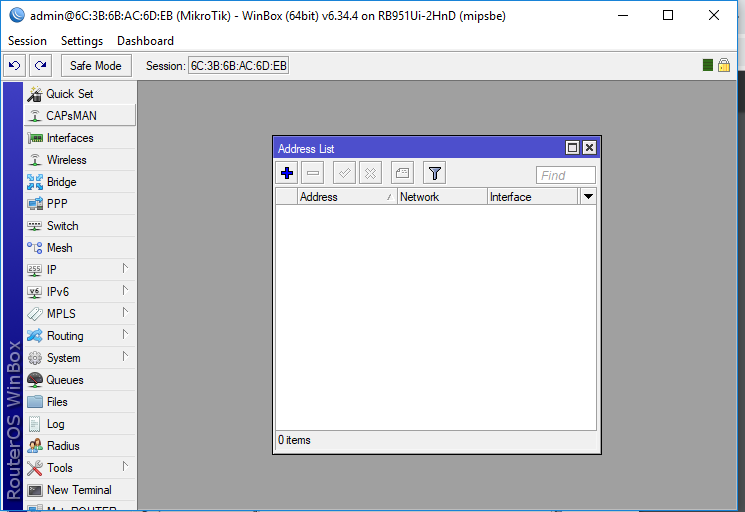
\includegraphics[scale=.5]{Capture2}
	\end{center}
	
\end{enumerate}

\end{document}